\section{Motorstyring }\label{sec:sec_motorstyring}
Målinger af vognens dynamik er baseret på stepresponset af vognen ved en konstant spænding, men med faste strømbegrænsninger.
\husk{JJ}{ref til afsnit om måling af vognens dynamic}
Dette giver anledning til at vægle en motorstyring der sørger for en styret strøm til motoren. 
Således vil udgangssignalet fra regulatoren i form af en regulering spænding, $V_{reg}$ omsættes i motorstyringen til $I_{reg}$, der igen giver den ønskede acceleration af vognen.  

\begin{itemize}
	\item Omsætter volt til ampere (current control)
	\item Pnp og npn transistorer med relativ høj strømrate
	\item Motor accelererer baseret på ampere. Volt angiver tophastighed.
	\item Min 1.25A maks 2.25A
\end{itemize}

\subsection{Design og dimensionering af motorregulering}
\husk{Kenneth}{Tekst rettes}
Da DC-motoren er en kompleks enhed, hvis dynamik og opbygning ligger uden for opfanget af denne rapport. 
Anvendes en simpel feedback regulering af strømmen igennem transistorerne, således at forholdet mellem indgangs signalet og udgangsstrømmen til motoren holdes konstant, som kan beskrives ved
\husk{JJ}{teoretisk model for motor styring}

I fig xx ses den valgte typografi af motor regulator.
\husk{JJ}{Diagram af motorstyring}

\husk{JJ}{Beskrivelse af motor regulator design} 
\husk{JJ}{Håndtering af transiente spændinger igennem bypass dioder}

\subsection{Beregninger}
\husk{JJ}{beregninger af forhold mellem spænding og strøm i regulatoren}
\husk{JJ}{PSpice simulering af regulator}

\subsection{Overførelsesfunktion af motor}
For at bestemme dynamikken af DC-motoren opstilles en forenklet model af motoren.

Ved at fastholde motoren, således at den elektromotoriske kraft kan sættes til nul, er det muligt at måle motores induktans.
\husk{JJ}{Model af DC-motor}
\begin{figure}[h!]
	\centering
	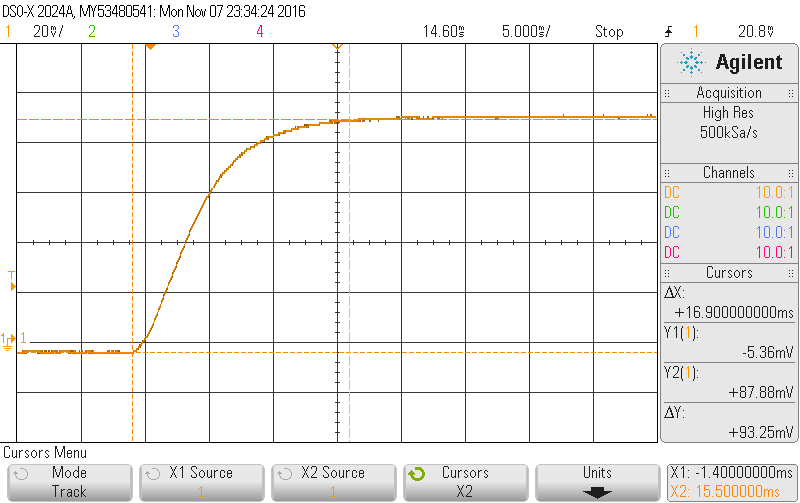
\includegraphics[width=.8\textwidth]{billeder/motor_L.png}
	\caption{Måling af transient forløb for strømmen igennem DC-motor.}
	\label{fig:motor_dynamik_scoop}
\end{figure}
\FloatBlock
Måling af strømmen igennem motoren er forstaget over en $0,2 \si{\ohm}$ test-modstand
\footnote{Modstanden med meget lille induktans}.
Motorens egen modstand er målt til $R_{motor} = 3,2 \si{\ohm}$, hvilket giver en semlet modstand på $R = R_{test} + R_{motor} = 3,4 \si{\ohm}$ i test opstillingen. 

Tidskonstanten for ladning af en spole er, $\tau = \frac{L}{R}$.
For at bestemme $L$, måles tiden $t$ ved $5\tau$ som er ved
\begin{align}
	\% opladning = \left( 1 - \frac{1}{e^{t/\tau}} \right) \cdot 100\% \Rightarrow  \left( 1 - \frac{1}{e^{t/5}} \right) \cdot 100 \approx 99,32\% 
\end{align}
derefter kan $L$ bestemmes som, ved aflæst tid på $16,9\si{\milli\second}$ i fig. \ref{fig:motor_dynamik_scoop} 
\begin{align}
	5\tau = \frac{L}{R} \Rightarrow L = 16,9\si{\milli\second} \cdot 3,4 \si{\ohm} = 57,5 \si{\milli\henry}
\end{align}


Overførelsesfunktion for motoren opstilles som
\begin{align}
H_{motor} = \frac{V_o}{V_i} = \frac{sL}{sL+R_{motor}} = \frac{ \frac{L}{R_{motor}}s}{ \frac{L}{R_{motor}}s +1} = \frac{\num{18E-3}s}{\num{18E-3}s +1}
\end{align}  


